%%%%%%%%%%%%%%%%%%%%%%%%%%%%%%%%%%%%%%%%%%%%%%%%%%%%%%%%%%%%%%%%%%%%%%%%%%%%%%%
%     STYLE POUR LES EXPOSÉS TECHNIQUES
%         3e année INSA de Rennes
%
%             NE PAS MODIFIER
%%%%%%%%%%%%%%%%%%%%%%%%%%%%%%%%%%%%%%%%%%%%%%%%%%%%%%%%%%%%%%%%%%%%%%%%%%%%%%%

\documentclass[a4paper,11pt]{article}

\usepackage{exptech}       % Fichier (./exptech.sty) contenant les styles pour
                           % l'expose technique (ne pas le modifier)


%\linespread{1,6}          % Pour une version destinée à un relecteur,
                           % décommenter cette commande (double interligne)

% UTILISEZ SPELL (correcteur orthographique) à accès simplifié depuis XEmacs


%\setlength{\parskip}{2ex}
\usepackage{color}
\usepackage{graphicx}
\usepackage{hyperref}
\hypersetup{
  bookmarks=true,         % show bookmarks bar?
  pdftitle={\'Etude pratique - Data carving},    % title
  pdfnewwindow=true,      % links in new window
  colorlinks=true,       % false: boxed links; true: colored links
  linkcolor=red,          % color of internal links (change box color with linkbordercolor)
  citecolor=green,        % color of links to bibliography
  filecolor=magenta,      % color of file links
  urlcolor=cyan           % color of external links
}
\definecolor{simColor}{rgb}{0.0, 0.5, 0.0}
\definecolor{dissimColor}{rgb}{0.8, 0.0, 0.0}
\definecolor{otherSimColor}{rgb}{0.0, 0.28, 0.67}

%%%%%%%%%%%%%%%%%%%%%%%%%%%%%%%%%%%%%%%%%%%%%%%%%%%%%%%%%%%%%%%%%%%%%%%%%%%%%%%

\title{ \textbf{Manuel utilisateur - BitGrapher} }
\markright{\'Etude pratique - Data carving}
                           % Pour avoir le titre de l'expose sur chaque page

\author{Alexandre \textsc{Audinot}, Thierry \textsc{Gaugry}, \\
        Nicolas \textsc{Hurman}, Gabriel \textsc{Prevosto} \\
        \\
        Encadrant : Gildas \textsc{Avoine}}

\date{}                    % Ne pas modifier

%%%%%%%%%%%%%%%%%%%%%%%%%%%%%%%%%%%%%%%%%%%%%%%%%%%%%%%%%%%%%%%%%%%%%%%%%%%%%%%

\begin{document}

\maketitle                 % Génère le titre
\thispagestyle{empty}      % Supprime le numéro de page sur la 1re page



\begin{abstract}
Nous possédons une multitude d'appareils que nous utilisons chaque jour, parfois à notre insu. Quelles informations enregistrent-ils ?
Ce document est le manuel utilisateur du logiciel développé au cours des études pratiques. Ce logiciel permet de comprendre la structure d'une mémoire de petite taille, comme on peut en trouver dans des cartes de transport, des abonnements de ski ou encore dans l'électronique embarquée de nos véhicules. En appliquant une série d'algorithmes et à travers une interface intuitive, disséquer ce type de support devient une tâche plus simple et accessible.
\end{abstract}

\section{Présentation de l'interface}
  L'interface utilisateur est découpée en 3 parties, qui reprennent les trois fonctionnalités clé du logiciel.

\begin{figure}[!h]
  \begin{center}
  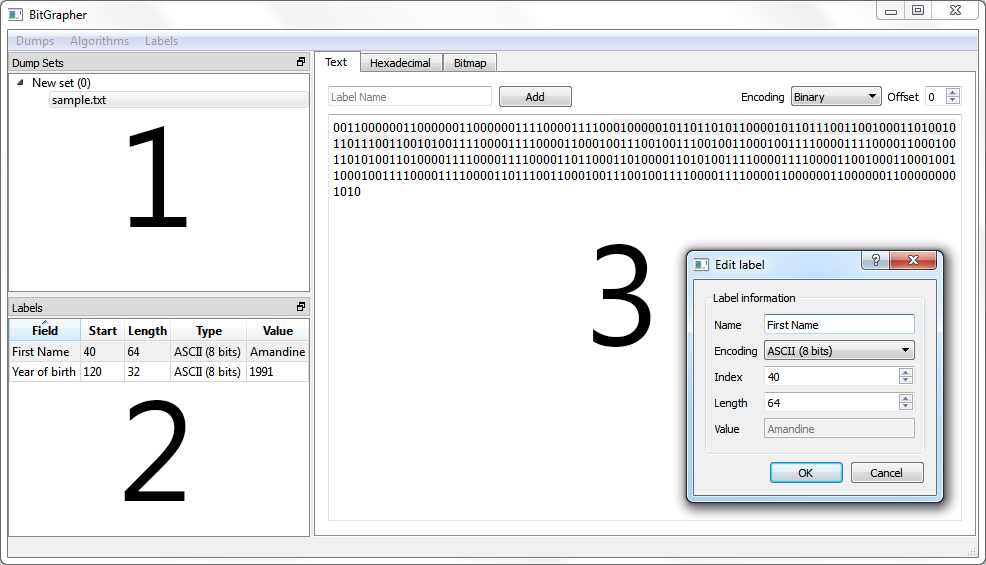
\includegraphics[width=\textwidth]{interface.png}
  \caption{Interface du logiciel}
  \label{interface}
  \end{center}
\end{figure}

Le premier volet (1) contient la liste des ensembles de dumps actuellement étudiés. Un dump set peut contenir plusieurs dumps, qui seront comparés entre eux. Cette partie sera traitée dans la partie Dumps & Set.

Le second volet (2) affiche la liste des champs identifiés par l'utilisateur. Au fur et à mesure de l'analyse du dump, les données collectées permettent de comprendre la structure du fichier.

La zone d'affichage principale (3) correspond à une visualisation des données du dump, qui peut être sous la forme de texte avec un encodage choisi au préalable comme sur la figure \ref{interface}, ou bien sous forme de bitmap.

Les menus donnent accès aux différents outils d'analyse, ainsi qu'à la sauvegarde et au chargement de dumps, de dump sets ou de masques.

L'interface utilisateur est entièrement fluide et les volets peuvent être détachés ou déplacés pour que l'utilisateur puisse organiser son espace de travail comme il le souhaite.

Une description complète du logiciel est disponible dans la documentation utilisateur, où se trouvent également les adresses de télechargement de versions compilées et prêtes à l'emploi pour Windows et Linux.

\section{Dumps \& Sets}
  Avant toute chose, il est nécessaire de créer ou d'ouvrir un set de dumps; un set de dumps correspond à un groupe de dumps qui seront ouvert en même temps. Nous appellerons "Set" les sets de dumps.
Un set peut donc servir soit de fichier "projet", pour réouvrir tout les dumps précédement utilisés, ou de groupe de dumps similaires.
Un set est un fichier avec l'extention .ds qui contient les adresses sur le disque des dumps à ouvrir; si vous avez une erreur au chargement d'un set, vérifiez si les dumps sont aux bons endroits.
Dans le cas de la création d'un set, il faudra le nommer (en cliquant dessus) puis lui rajouter des dumps. Cela s'effectue en cliquant sur "Dumps/Add Dump".
Il peut arriver qu'un fichier se retrouve par erreur dans un set, ou qu'il ne soit plus nécessaire; la fonction Remove Dump du menu Dump permet de retirer du set le dump sélectionné.
Les fonctions "Save set" et "Save set as ..." du menu Dump permettent de sauvegarder un set, pour pouvoir reprendre le travail plus tard sur les mêmes données. Un set ne contients que les positions des Dumps, veillez à ne pas déplacer vos dumps ou les supprimer, ou vous risqueriez de provoquer des erreurs !
Un click sur un autre dump actualise l'interface avec ces nouvelles données.
\section{Vues}
  Les vues sont accessibles via les différents onglets. Il y a 3 vues différentes :
\begin{description}
  \item[Text] \hfill \\
  Elle permet de visualiser l'intégralitée du dump sous l'encodage spécifié dans le selecteur "Encoding". Le décalage peut être géré via la case Offset. Le bouton Add et de la case Label Name permettent d'ajouter de nouveaux labels. Leur fonctionnement détaillé est décrit dans la partie Labels.
  
  \item[Hexadecimal] \hfill \\
  Elle permet de visualiser le dump sous forme hexadécimale. L'offset est visible sur la gauche. Cette vue permet entre autre de repérer les motifs qui se répètent, tels que les séparateurs.

  \item[Bitmap] \hfill \\
  Elle permet de visualiser le dump courant sous forme de carrés de couleur. Cette vue permet entre autre de repérer les morceaux qui se répètent.
\end{description}

Chaque vue affiche le dump courant, c'est à dire le dump en surbrillance dans la zone Dumps Sets. Il est possible de changer de vue en cliquant sur l'onglet voulu.


\section{Labels}
  Cette zone contient un tableau des morceaux de dump déjà décodés. Cette zone est intimement liée au menu Labels.

Pour ajouter un nouveau champ, il faut sélectionner la zone avec le curseur de la souris dans la vue texte, puis lui définir un nom. L'appui sur le bouton Add ajoute au tableau des labels une entrée avec le nom saisi, la zone définie par la souris et l'encodage courant.
Si une erreur s'est glissée dans vos données, vous pouvez :
\begin{description}
	\item[Editer la ligne] \hfill \\
	il suffit de double cliquer dessus. La fenètre Edit Label (figure \ref{editlabel}) s'affiche alors. Il n'y a plus qu'a renseigner les informations correctes. A noter que le champ "Value" n'est pas éditable et ne sert qu'a vérifier les informations.
	
	\begin{figure}[!h]
		\begin{center}
		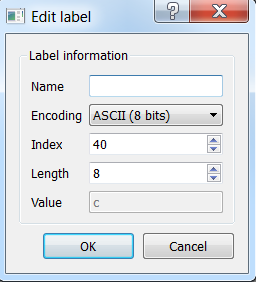
\includegraphics[width=\textwidth]{Edit_label.png}
		\caption{Fenètre d'édition des labels}
		\label{editlabel}
		\end{center}
	\end{figure}
	
	\item[Supprimer la ligne] \hfill \\
	Cette action est disponible en cliquant sur "Labels/Remove Label".

\end{description}
 
 Une fois l'analyse terminée, il convient de sauvegarder les données trouvées. Les fonctions "Labels/Save Mask" et "Labels/Save Mask as ..." permettent d'enregistrer le tableau de labels sous forme d'un masque; c'est à dire uniquement les données indépendantes du Dump, pour qu'il soit réutilisable.
 Les masques ainsi créés peuvent être ouvert et utilisé grâce à la fonction "Labels/Open Mask". Leur format est détaillé dans la documentation technique du projet, dans le cas où vus voudriez créer un masque à partir de spécifications techniques. Il n'est cependant nullement nécessaire de savoir cette information pour utiliser le logiciel.
\section{Menu d'aide à la décision : Algorithms}
  Parfois, les outils classiques ne suffisent plus; il y a alors besoin d'utiliser des méthodes mathématiques poussées pour obtenir de l'information. Deux de ces algorithmes sont implémentés dans BitGrapher :
  \subsection{Fonction Similarities} \label{Similarities} Cette fonction, accessible via le menu Algorithms, permet mettre en évidence les chaînes de bits semblables au même endroit dans un dump.

Dans le cas de deux dumps, les similarités sont représentées par la couleur verte, tandis que les similarités sont représentées par la couleur rouge. Un exemple de similarités est représenté sur la figure \ref{04-1-sim_simple}. Pour faciliter la compréhension, on y a remplacé les bits (de sens à priori inconnu) par des lettres.

\begin{figure}[!h]
  \begin{center}
  {\tt\center
  {Dump 1 : \color{simColor} Ce}{\color{dissimColor} ci es}{\color{simColor}t }{\color{dissimColor} un exemple de }{\color{simColor} similarité}

  {Dump 2 : \color{simColor} Ce}{\color{dissimColor} la me}{\color{simColor}t }{\color{dissimColor} en couleur la }{\color{simColor} similarité}
  }
  \end{center}
  \caption{Exemple de similarités}
  \label{04-1-sim_simple}
\end{figure}

Afin d'affiner la recherche, il est possible de spécifier une taille de chaîne minimum, comme l'illustre la figure \ref{04-1-sim_taille_min}.

\begin{figure}[!h]
  \begin{center}
  {\tt
  {Dump 1 : \color{dissimColor} Ceci est un exemple de }{\color{simColor} similarité }{\color{dissimColor} avec une taille minimum de 4}

  {Dump 2 : \color{dissimColor} Cela met en couleur la }{\color{simColor} similarité }{\color{dissimColor} faisant plus de 4 caractères}
  }
  \end{center}
  \caption{Similarités avec une taille de chaîne minimum}
  \label{04-1-sim_taille_min}
\end{figure}


Dans le cas de plusieurs dumps, on dispose de trois couleurs. Le rouge représente les dissimilarités, le vert les similarités concernant le dump visualisé (c'est-à-dire les similarités commune à ce dump et à d'autres), tandis que le bleu correspond aux similarités ne concernant pas le dump visualisé (c'est-à-dire les similarités communes à d'autres dumps).
Ces couleurs ont des nuances : plus le vert ou le bleu sont prononcés, plus il y a de dumps partageant la similarité en question. La figure \ref{04-1-sim_mult} est un exemple de similarités avec 3 dumps.

\begin{figure}[!h]
  \begin{center}
  {\tt
  {Dump 1 : \color{dissimColor} Encore un}{\color{otherSimColor} e au}{\color{dissimColor} tre }{\color{simColor} similarité}{\color{dissimColor} .}

  {Dump 2 : \color{dissimColor} Toujours }{\color{simColor} plus }{\color{dissimColor} de }{\color{simColor} similarité}{\color{dissimColor} s}

  {Dump 3 : \color{dissimColor} colorées }{\color{simColor} plus }{\color{dissimColor} qu'}{\color{otherSimColor} auparavant}{\color{dissimColor} .}
  }
  \end{center}
  \caption{Similatités entre trois dumps}
  \label{04-1-sim_mult}
\end{figure}
  \subsection{Fonction Dot Plot Pattern} \label{Dot_Plot_Pattern} Cette fonction, accessible via le menu Algorithms, permet d'afficher les segments ressemblants entre deux dump sous forme de graphe. Il faut en premier lieu cliquer sur Dot Plot Pattern dans le menu Algorithms. Une fenètre s'affiche alors :

\begin{figure}[!h]
  \begin{center}
  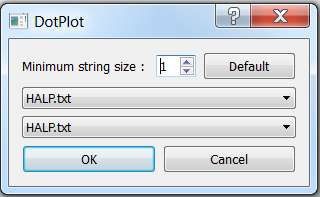
\includegraphics[scale=1]{dotplotdialog.png}
  \caption{Fenetre de lancement du Dot Plot Pattern}
  \label{dotplotdialog}
  \end{center}
\end{figure}

Il faut alors sélectionner une \emph{Minimum String Size}; il s'agit de la taille minimale que les blocs de données identiques doivent avoir pour apparaitre. Si vous avez peu de diagonales sur votre Dot Plot Pattern, c'est peut-être que vous avez sélectionné une taille de diagonale trop grande. Le bouton \emph{Default} permet d'entrer une taille qui promet statistiquement de bons résultats.
Les deux champs suivant permettent de sélctionner les deux dumps qui seront utilisés lors du Dot Plot Pattern. Le premier dump se retrouvera en abscisse, et le second en ordonnée. Il est possible d'utiliser deux fois le même dump, pour voir les motifs se répétant au sein d'un même dump.

Après appui sur le bouton \emph{OK}, on obtient la fenètre suivante :
\begin{figure}[!h]
  \begin{center}
  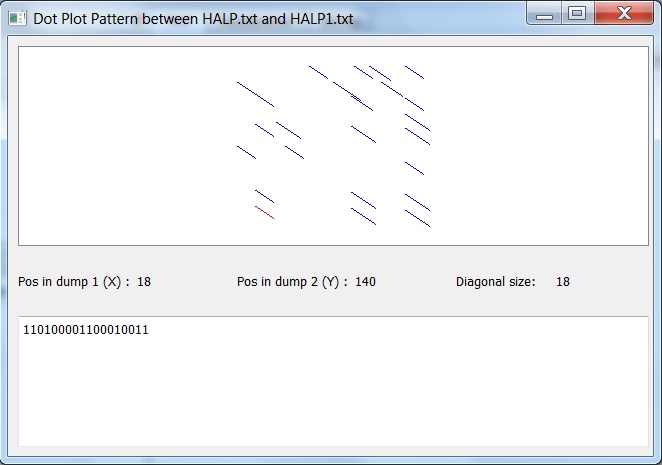
\includegraphics[scale=1]{dotplotpatternview.png}
  \caption{Fenetre du Dot Plot Pattern}
  \label{dotplotpattern}
  \end{center}
\end{figure}

Un click sur une diagonale la sélectionne; elle devient rouge et le bas de l'interface est actualisée avec les informations relative à celle-ci :
\begin{description}
\item[Pos in dump 1 (X)] \hfill \\
	Indique le numéro du bit où commence la ressemblance dans le premier dump, 0 correspondant au début de fichier.
	
\item[Pos in dump 2 (Y)] \hfill \\
	Indique le numéro du bit où commence la ressemblance dans le deuxième dump, 0correspondant au début de fichier.

\item[Diagonal Size] \hfill \\
	Indique la longueur de la diagonale, ce qui correspond au nombre de bits en commun de suite entre les deux dumps.
	
\item[La zone de texte en bas] \hfill \\
	Elle contient la chaine de bits commune aux deux dumps.

\end{description}

Si les deux dumps disposent de champs identiques aux mêmes endroits, il y a alors des diagonales au centre du graphe. Si les deux dumps sont identiques, alors une diagonale centrale faisant la longueur du dump est visible.
\section{Contacts}
  Si vous avez des questions ou des remarques, vous pouvez nous contacter par mail :

Alexandre \textsc{Audinot} - alexandre.audinot@insa-rennes.fr
Thierry \textsc{Gaugry} - thierry.gaugry@insa-rennes.fr
Nicolas \textsc{Hurman} - nicolas.hurman@insa-rennes.fr
Gabriel \textsc{Prevosto} - gabriel.prevosto@insa-rennes.fr
\newpage

\end{document}
